\section{Justficación}
Los datos presentados en \cite{ODS23} muestran que menos de la mitad del agua residual generada es tratada de manera adecuada, sobre todo en la región hidrológica Lerma-Santiago donde se tiene un deficiente control de las zonas de descarga de las redes colectoras, vertiendo la mayoría en cuerpos de agua superficiales generando problemas sanitarios en poblaciones que no cuentan con plantas potabilizadoras (como es el caso de Lagos de Moreno) \citep{CEAJ2015}.\par
Por tal motivo resulta esencial el fomentar la investigación en técnicas de tratamiento de aguas residuales con vistas a reducir la carga de contaminantes de los cuerpos de agua y generar una recarga artificial de los acuíferos, reduciendo el déficit de agua al que se enfrentan actualmente los acuíferos del país y proponiendo un sistema capaz de satisfacer las necesidades de la población a un bajo coste y con mayor eficiencia de trabajo.\par
Actualmente ya se cuenta con varios modelos, siendo los \gls{ASM} los más representativos y respaldados, contando con varios trabajos de investigación que demuestran la concordancia entre los datos reales y las predicciones generadas por el modelo.\par
\begin{figure}[H]
	\centering
	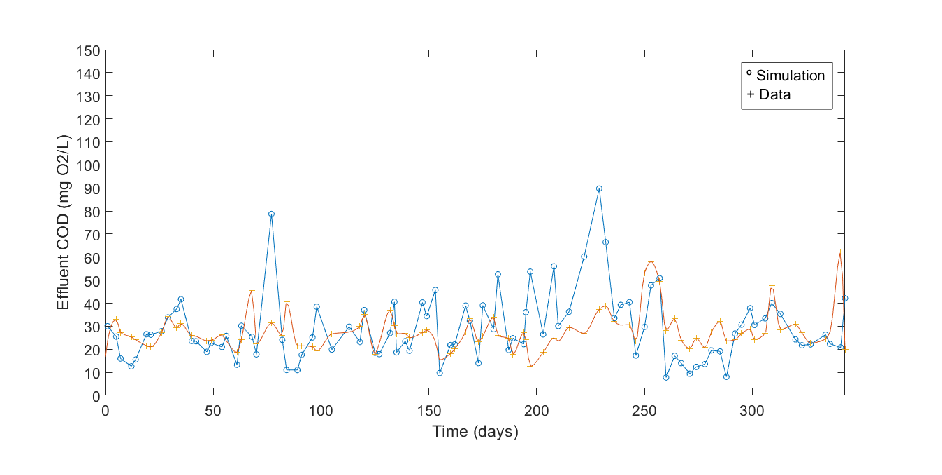
\includegraphics[scale=.95]{../Images/Costa22_sim.pdf}
	\\\small{Fuente: \cite{Costa2022}}
	\caption{Gráfica comparativa entre los datos obtenidos por simulación mediante el modelo \acrshort{ASM}1 y los datos analizados por el autor de la \acrshort{PTAR} de Salamanca España, en dónde Y\textsubscript{\textit{H}} = 0.6 y \unichar{"00B5}\textsubscript{\textit{H,max}} = 0.4 d\textsuperscript{-1} resultan los valores que menor error promedio presentan en la comparativa (-0.5\% de error para ser más específicos)}\label{fig:sim-costa}
\end{figure}
\cite{Costa2022}, realiza una comparación entre la aplicación del modelo \acrshort{ASM}1 y la \acrshort{PTAR} de Salamanca España, concluyendo que, aunque el modelo realiza predicciones que llegan a acercarse al resultado in-situ, es necesario que se realicen ajustes a los parámetros \textit{\unichar{"00B5}}$_{H,max}$ y $Y_{H}$ con el fin de conseguir una mejor representación y reducción del error promedio entre los valores de simulación y los datos analizados (ver figura \ref{fig:sim-costa}). También destaca que, si bien el modelado matemático no es capar de predecir la variabilidad generada inevitablemente con respecto a las fluctuaciones en las condiciones de operación a las que son sometidas las comunidades bacterianas dentro del sistema, este proceso sirve para comprender las causas de tales variaciones y como afectan al sistema de manera general con el fin de seguir mejorando el modelo, ya que como lo menciona el autor, el modelo original fue publicado hace mas de 30 años y , aunque se han desarrollado modelos que solventan errores u omisiones del primer modelo, estos están aún lejos de tener errores entre el valor simulado y el analizado in-situ.\par
En otro articulo, \cite{Gernaey04} hablan acerca de las aplicaciones que presenta el modelado en distintos ámbitos, resaltando tres casos:
\begin{enumerate}
	\item \textbf{Simulación con fines educativos:} en dónde se busca que el operador comprenda de forma detallada el funcionamiento del sistema de lodos activados y las implicaciones que generan los cambios en las condiciones operativas, variaciones climáticas y problemas adversos típicos relacionados al ciclo metabólico de las comunidades microbiológicas presentes en el sistema.
	\item \textbf{Simulación con fines de diseño:} buscando en este apartado analizar todos los escenarios posibles para resolver ciertas problemáticas adjuntas a cada caso de estudio, reduciendo costos significativos y tiempo en el escalado entre un sistema de pruebas a nivel laboratorio y la planta piloto. Este punto va de la mano con el siguiente punto, el cual habla de;
	\item \textbf{Simulación para la optimización de procesos:} refiriendo a esto la necesidad de realizar mejoras operativas respecto a nuevas exigencias debido a cambios en el volumen y carga de contaminantes que entran a la \acrshort{PTAR} ya en servicio; y/o a deficiencias no analizadas durante la fase de diseño que salen a la luz una vez  la \acrshort{PTAR} entra en operación.
\end{enumerate}
Por otra parte, \cite{Petersen2002} profundiza en la importancia que tiene el proceso de calibración al momento de que se utilizan estos modelos, analizando las diferentes variables operativas para una \acrshort{PTAR} con \gls{efluente} del tipo municipal-industrial, advirtiendo la importancia de una buena interpretación de todo el sistema al momento de realizar dicha calibración, ya que puede cometerse el error de utilizar modelos calibrados tomando en cuenta solamente los datos para cuando la planta esta en un sistema estacionario, lo cual genera errores asociados a las mismas variaciones de un sistema que normalmente se encuentra en un estado dinámico.